\subsection{Nativer Mobile Client}

Mit IP5 wurde bereits ein Client umgesetzt.
Dieser muss für IP6 migiert werden.
Hier wird beschrieben, wie die bestehenden Anforderungen mit dem nativen client umgesetzt werden können.

\subsubsection{Benutzeroberfläche}

Die Ansichten zur Anmeldung und Zimmerauswahl werden analog zum bestehenden Mobile Client umgesetzt.
Die Login Seite beinhaltet einen kurzen Willkommenstext und ein Logo für Praxisruf.
Darunter findet sich ein einfaches Formular zur Eingabe von Benutzername und Passwort.

\begin{figure}[h]
    \centering
    \begin{minipage}[b]{0.4\textwidth}
        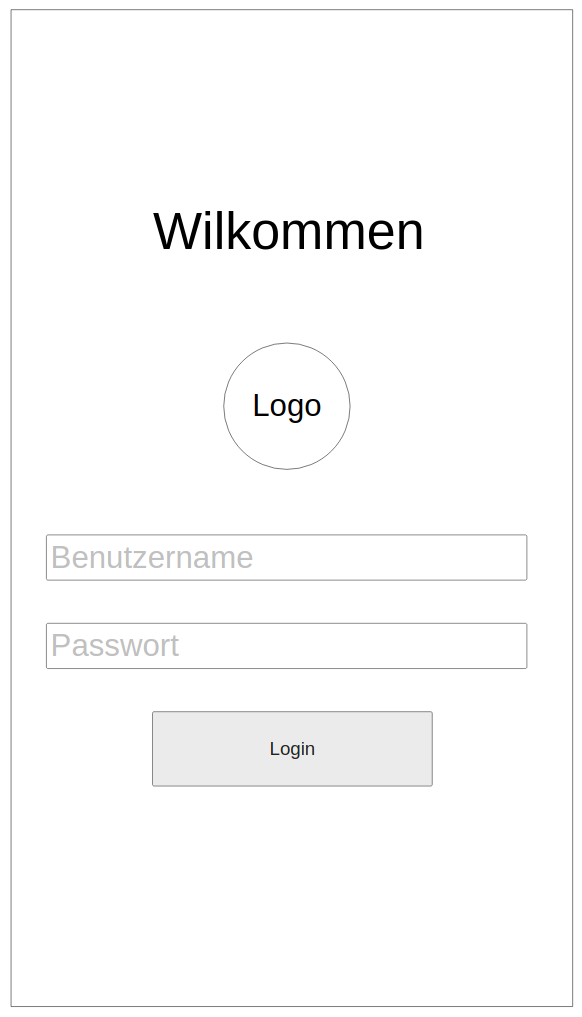
\includegraphics[width=\textwidth]{/home/joshua/FHNW/dev/IP6/IP6_Bachelorarbeit_Bericht_Cloudbasiertes_Praxisrufsystem/src/graphics/mockups/mockup_login}
        \caption{Mockup Login}
    \end{minipage}
    \hfill
    \begin{minipage}[b]{0.4\textwidth}
        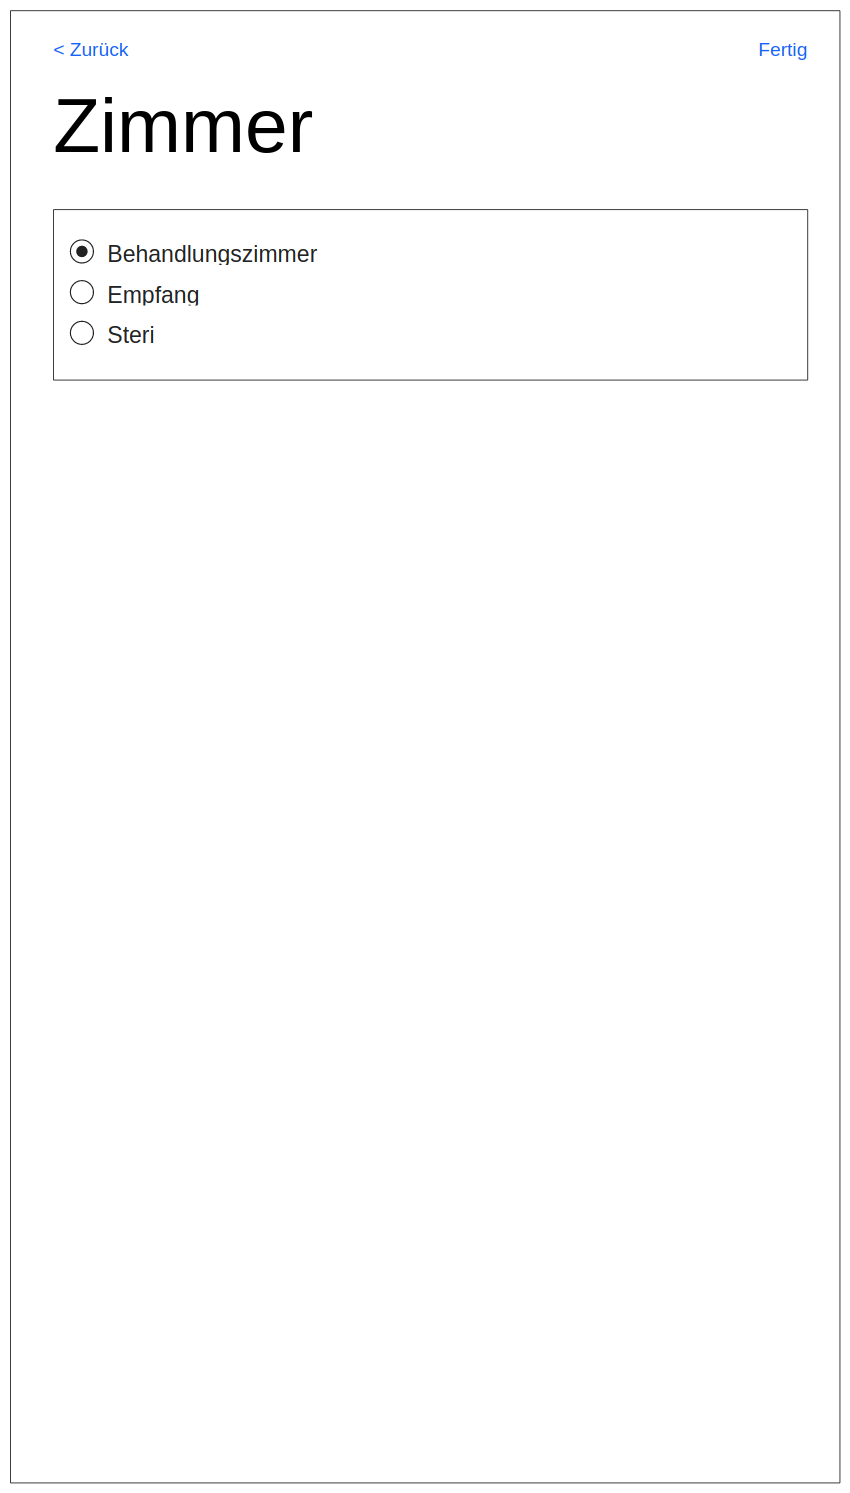
\includegraphics[width=\textwidth]{/home/joshua/FHNW/dev/IP6/IP6_Bachelorarbeit_Bericht_Cloudbasiertes_Praxisrufsystem/src/graphics/mockups/mockup_clientselect}
        \caption{Mockup Zimmerwahl}
    \end{minipage}\label{fig:Mockups-Login-ClientSelection}
\end{figure}

Die Zimmerauswahl besteht aus einem Seitentitel und einem Panel indem das gewünschte Zimmer ausgewählt werden kann.
In der Auswahl sind alle Zimmer zu sehen, welche dem Benutzer zur Verfügung stehen.
In der Kopfzeile sind die Schaltflächen ''Zurück'' und ''Fertig'' zu sehen.
Die Schaltfläche ''Zurück'', bricht die Anledung ab und führt zurück auf die Login Ansicht.
Die Schaltfläche ''Fertig'' bestätigt die Auswahl und leitet zur Hauptansicht weiter.
Wird bestätigt, ohne dass ein Zimmer angewählt ist, wird dem Benutzer eine Fehlermeldung angezeigt und nicht zur Hauptansicht weitergeleitet.

\clearpage

In der Hauptansicht gliedert sich in die Bereiche Home, Inbox und Einstellungen.
Zwischen den drei Bereichen kann über eine Leiste am unteren Ende des Bildschirms navigiert werden.
Die Ansicht Home zeigt dem Benutzer die Buttons, über welche er Meldungen versenden und Anrufe in der Gegensprechanlage starten kann.
Wird ein Anruf gestartet, wird die Ansicht für aktive Anrufe angezeigt.
Diese zeigt dem Benutzer den Titel des gestarteten Anrufs, sowie eine Liste aller Teilnehmer zusammen mit dem Verbindungsstatus jedes Teilnehmers.
Der Titel des Anrufes entspricht dem Anzeigetext des entsprechenden Buttons für ausgehende Anrufe und dem Namen des Anrufers für empfangene Anrufe.
Neben den Anrufinformationen zeigt die Ansicht für aktive Anrufe drei Buttons.
Über diese können Microfon und Lautsprecher des eigenen Gerätes stummgeschaltet werden.
Weiter kann über der Anruf über den dritten Button beendet werden.
Nach einem beendeten Anruf, wird zurück auf die Hauptansicht weitergeleitet.
Für den Anrufern ist das immer der Home Bereich.
Für den Empfänger entspricht es dem Bereich, der vor dem Empfang des Anrufes angezeigt wurde.

\begin{figure}[h]
    \centering
    \begin{minipage}[b]{0.4\textwidth}
        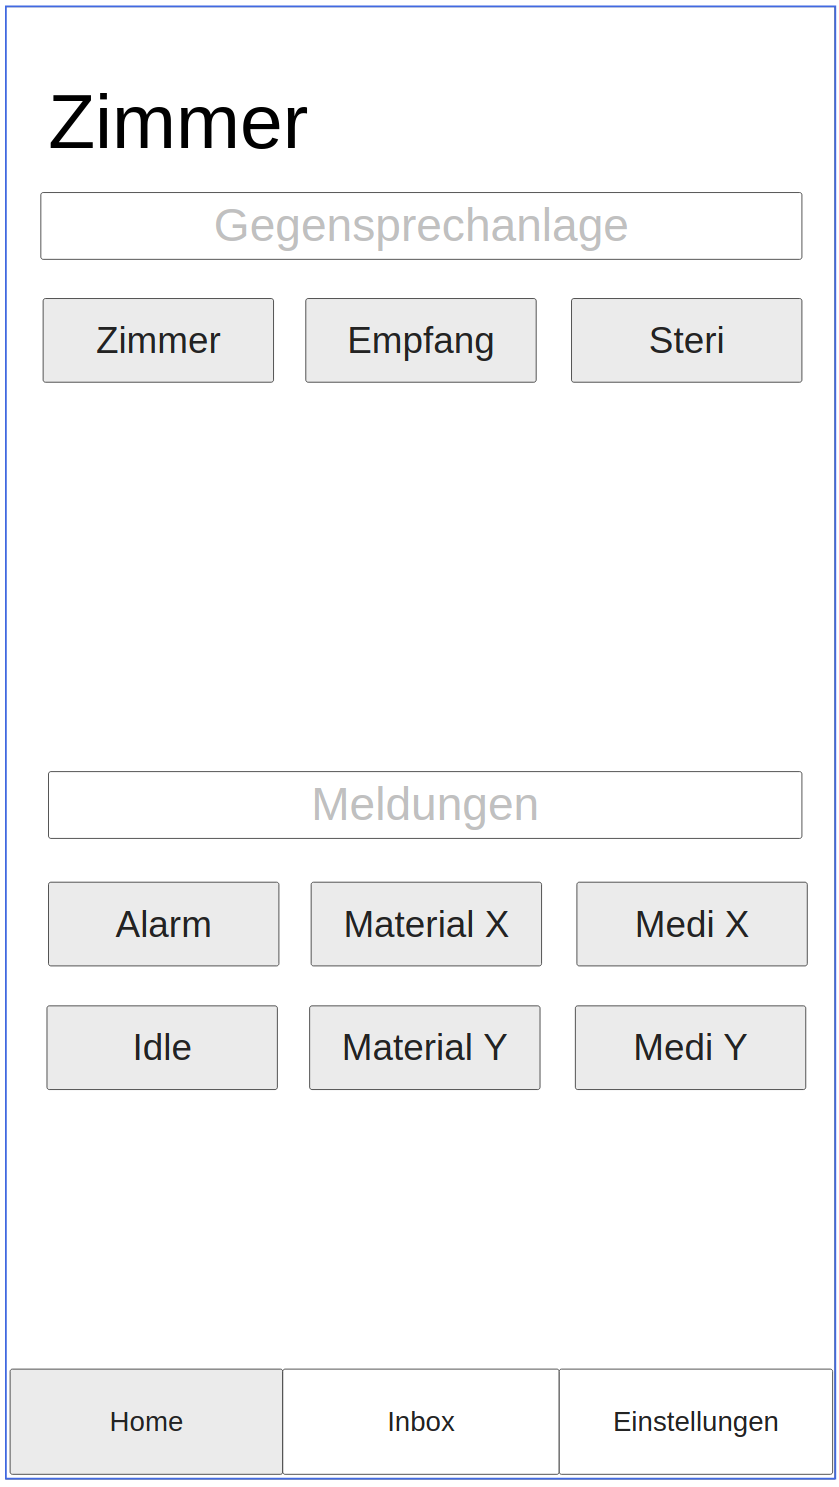
\includegraphics[width=\textwidth]{/home/joshua/FHNW/dev/IP6/IP6_Bachelorarbeit_Bericht_Cloudbasiertes_Praxisrufsystem/src/graphics/mockups/mockup_intercom}
        \caption{Mockup Home}
    \end{minipage}
    \hfill
    \begin{minipage}[b]{0.4\textwidth}
        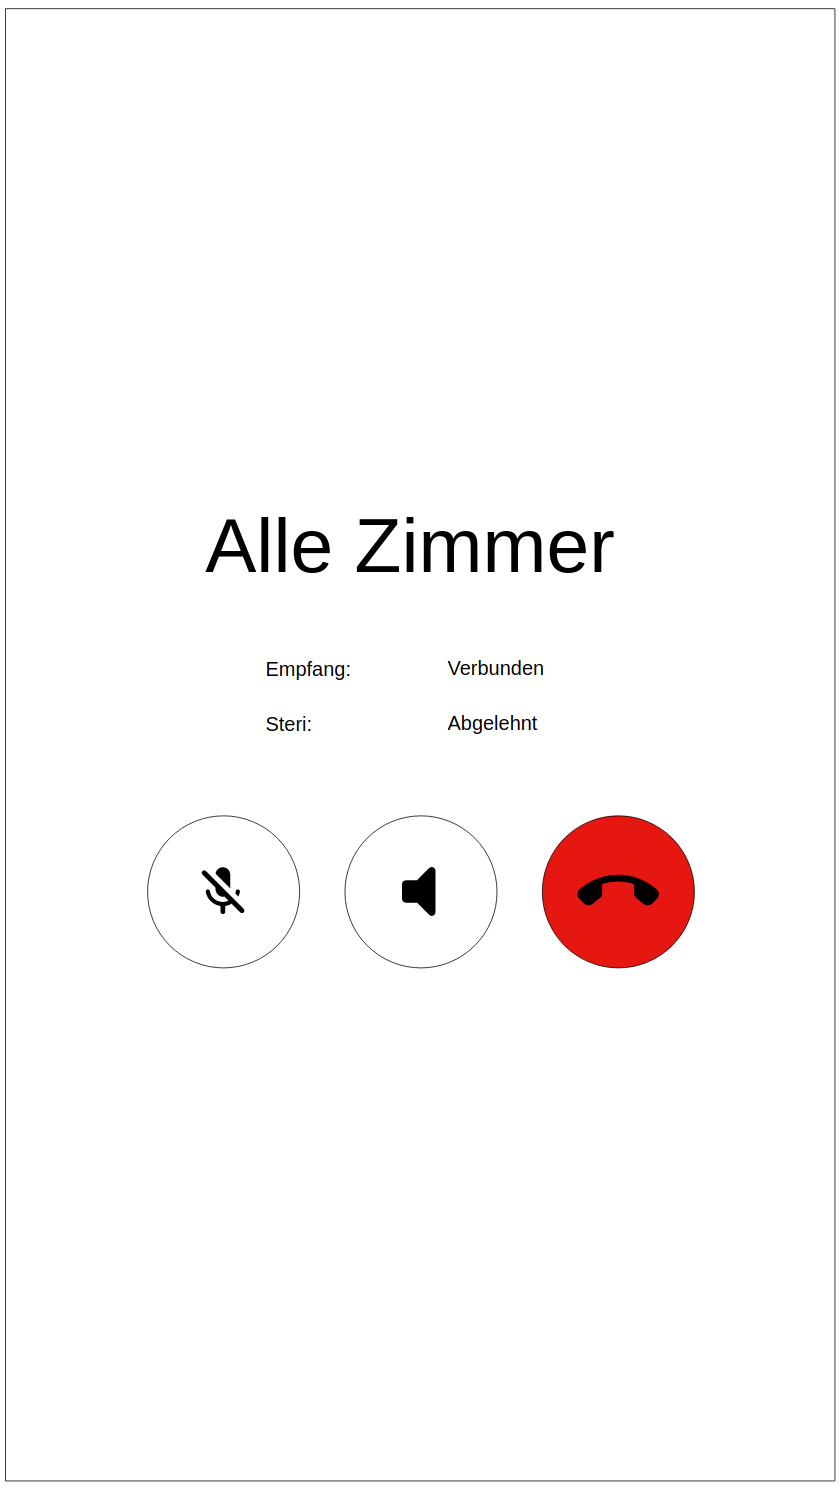
\includegraphics[width=\textwidth]{/home/joshua/FHNW/dev/IP6/IP6_Bachelorarbeit_Bericht_Cloudbasiertes_Praxisrufsystem/src/graphics/mockups/mockup_call}
        \caption{Mockup Aktiver Anruf}
    \end{minipage}\label{fig:Mockups-Home-ActiveCall}
\end{figure}

Der Bereich Inbox zeigt eine Liste der empfangenen Meldungen sowie der empfangenen und verpassten Anrufe.
Für Meldungen wird der Titel der Benachrichtigung gefolgt vom Namen des Versenders in Klammern sowie der Haupttext der Meldung angezeigt.
Für Anrufe wird der Name des Anrufers und ein Text der besagt ob es sich um einen empfangenen, verpassten oder abgelehnten Anruf handelt angezeigt.
Einträge für Meldungen sowie verpasste und abgelehnte Anrufe müssen durch antippen quittiert werden.
Solange unquittierte Meldungen oder Anrufe in der Inbox sind ertönt, wird im Abstand von 60 Sekunden eine Benachrichtigung angezeigt, die den Benutzer erinnert, die Inbox zu quittieren.
Der Bereich Settings zeigt den Namen des aktuellen Benutzers und ausgewählten Zimmers.
Über die Schaltfläche Abmelden, kann sich der Benutzer aus der Applikation abmelden.
Die Schaltfläche Benachrichtigungen vorlesen ist standardmässig aktiviert.
Wird die Option deaktiviert, werden Benachrichtigungen nie vorgelesen.
Die Schaltfläche Anruge empfangen ist ebenfalls standardmässig aktiviert.
Wird diese Option deaktiviert, werden alle empfangenen Anrufe automatisch abgelehnt und stattdessen eine Benachrichtigung angezeigt.
Ausgehende Anrufe können auch getätigt werden, wenn diese Option aktiviert ist.


\begin{figure}[h]
    \centering
    \begin{minipage}[b]{0.4\textwidth}
        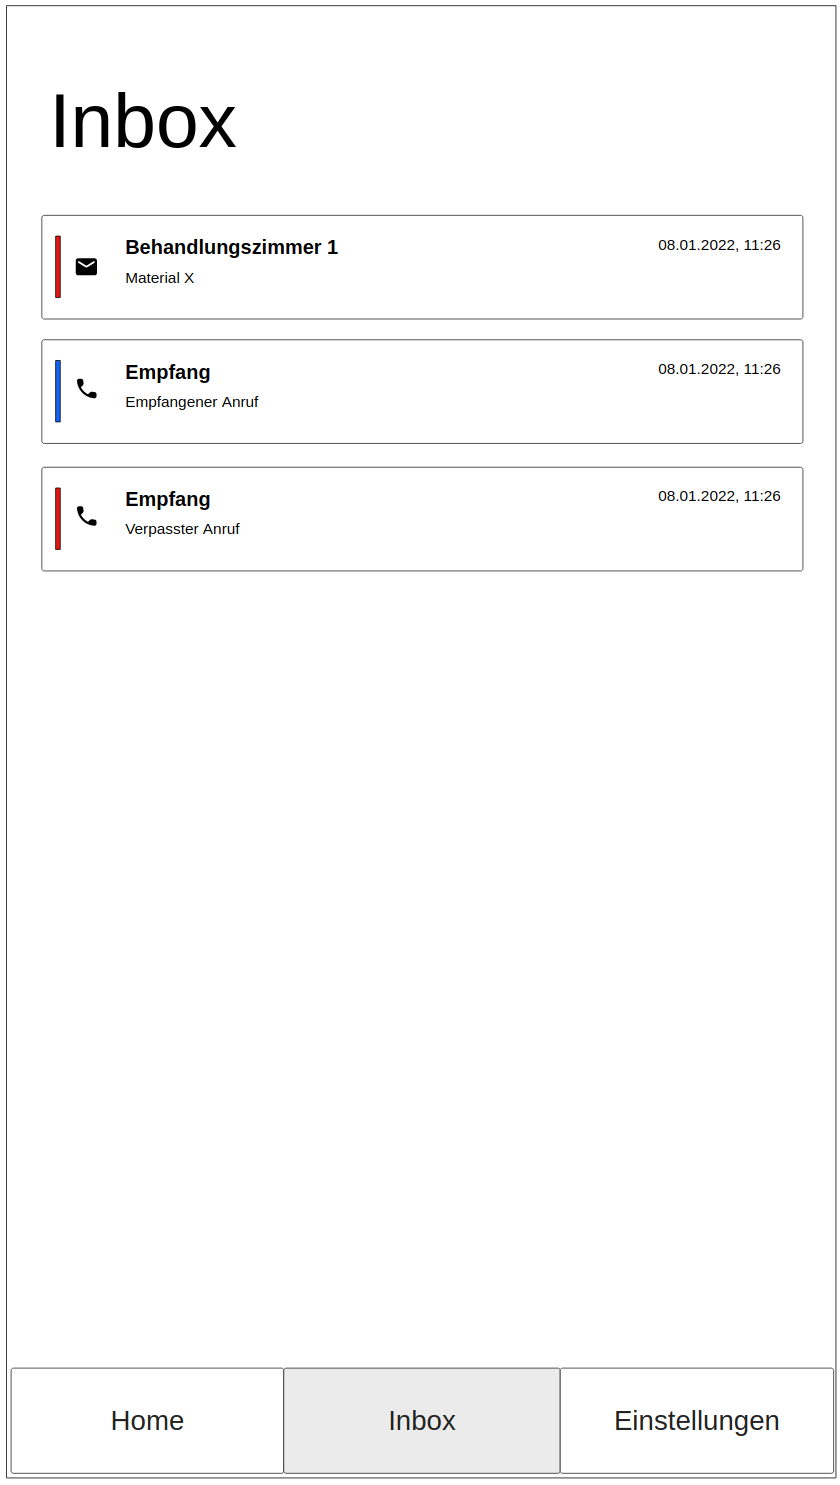
\includegraphics[width=\textwidth]{/home/joshua/FHNW/dev/IP6/IP6_Bachelorarbeit_Bericht_Cloudbasiertes_Praxisrufsystem/src/graphics/mockups/mockup_inbox}
        \caption{Mockup Inbox}
    \end{minipage}
    \hfill
    \begin{minipage}[b]{0.4\textwidth}
        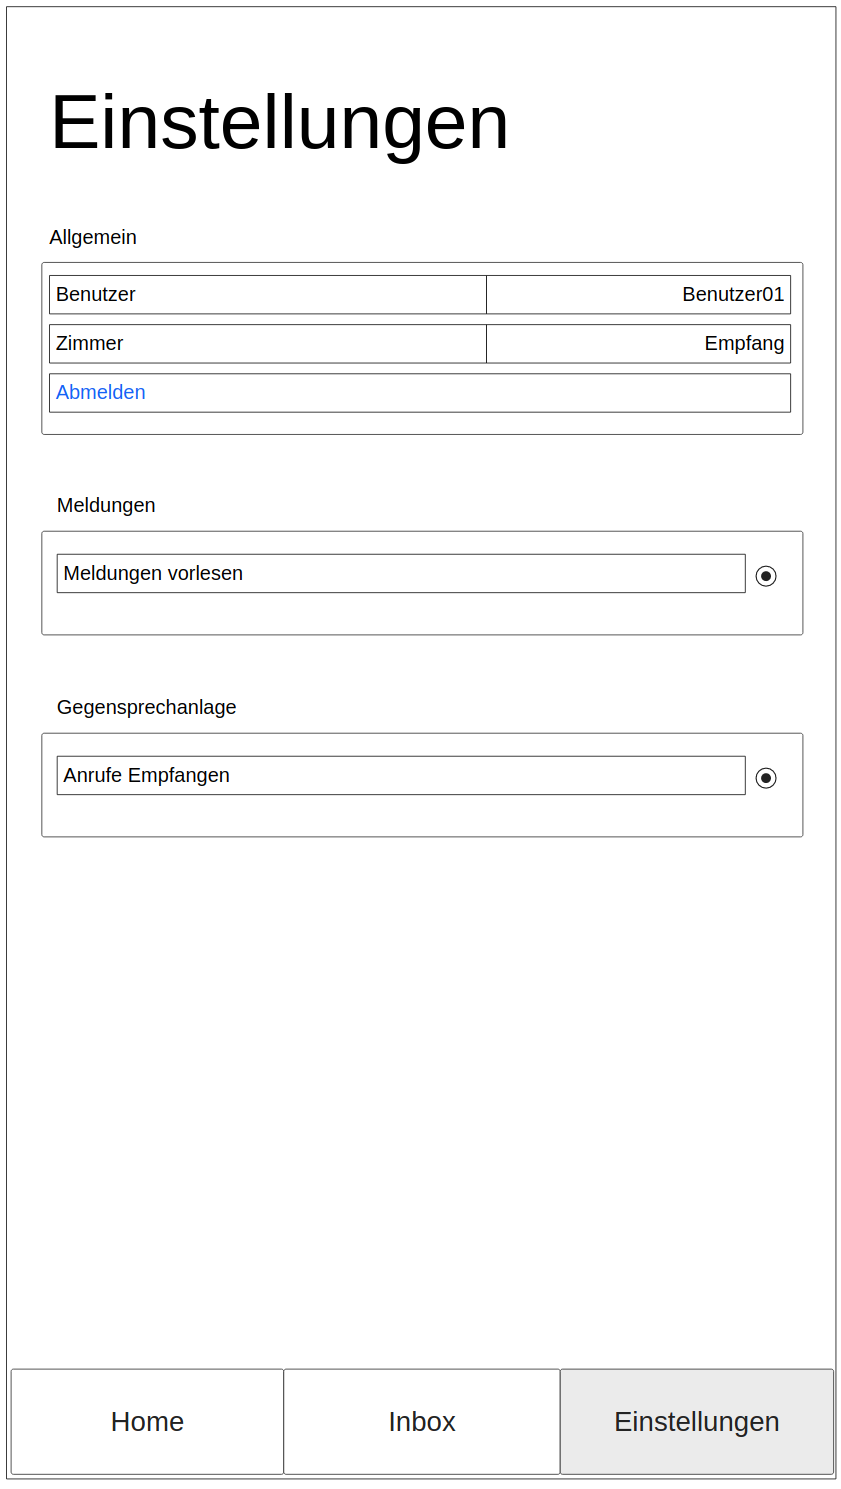
\includegraphics[width=\textwidth]{/home/joshua/FHNW/dev/IP6/IP6_Bachelorarbeit_Bericht_Cloudbasiertes_Praxisrufsystem/src/graphics/mockups/mockup_settings}
        \caption{Mockup Einstellungen}
    \end{minipage}\label{fig:Mockups-Inbox-Settings}
\end{figure}

\subsubsection{Anbindung CloudService}

Der Mobile Client muss an die API des Cloudservices angebunden werden.
Es wird eine Anbindung an die Domäne Configuration zur Anmeldung und Auswahl des gewünschten Zimmers, an die Domäne Notification zum Versenden von Benachrichtigungen und an die Domäne Speech Synthesis für den Bezug von Sprachdaten benötigt.
Die Schnittstellen dieser Domänen stehen als REST Endpoints zur verfügung.
In diesem Unterkapitel wird beschrieben, wie REST Aufrufe im nativen iOS Client integriert werden sollen.\footnote{Die Anbindung der Domäne Signaling findet nicht über REST statt und ist im Kapitel 5.2.4 beschrieben.}

Die Basisbibliothek für iOS Entwicklung bietet die Klasse URLSession, über welche Netzwerkaufrufe getätigt werden können.
Über URLSession.shared steht zudem eine Standard Instanz zur Verfügung, über welche Anfragen erstellt werden können.\cite{ios_urlsession}
Die Klasse UrlRequest ermöglicht es, Http-Request für eine URL mit Header und Body zu erstellen.\cite{ios_urlrequest}
Um die Integration dieser Klassen in den Mobile Client zu vereinfach, wird ein zentraler Service mit dem Namen PraxisrufApi erstellt.
Dieser kapselt das Erstellen, Befüllen und Absetzten der nötigen UrlRequest Instanzen und bietet öffentliche für die Http Verben Get, Post und Delete an.

Der Basis des Api Service lädt die Basis URL für die Praxisruf API us der Umgebungskonfiguration.
Die http Methoden auf dem Basis Service nehmen eine subUrl für den Aufruf entgegen.
Diese wird der Basis Url angehängt.
Post und Put nehmen zudem einen Parameter data für den Inhalt des Request Bodies entgegen.
Aus diesen Informationen kann der Http Request gebaut und versendet werden.
Als letzten Parameter nehmen alle Methoden einen Parameter mit dem Namen completion entgegen.
Dabei handelt es sich um ein Callback, welches beim Erfolg oder Fehlschlagen der Anfrange an die API ausgeführt wird.

\begin{figure}[h]
    \centering
    \begin{minipage}[b]{0.8\textwidth}
        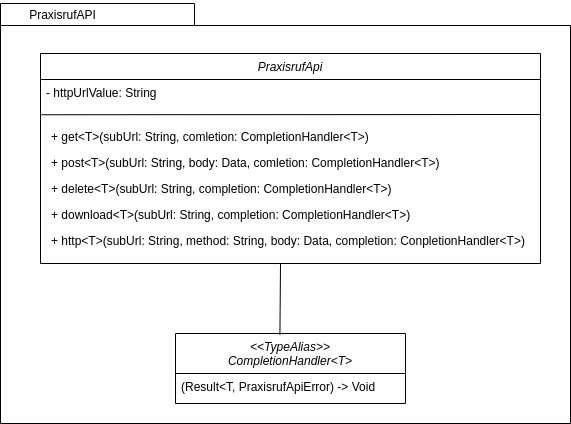
\includegraphics[width=\textwidth]{/home/joshua/FHNW/dev/IP6/IP6_Bachelorarbeit_Bericht_Cloudbasiertes_Praxisrufsystem/src/graphics/diagramms/Class_PraxisrufAPI_V01}
        \caption{Klassendiagramm PraxisrufAPI}
    \end{minipage}
\end{figure}


%\lstinputlisting[caption=PraxisrufApi.swift,language=java,label={lst:praxisrufapi.swift}]{listings/praxisrufapi.swift}

Als Input Paramter dieses Callbacks wird immer der Typ Result<T, PraxisrufApiError> verwendet.
Bei Result handelt es sich um einen Wrapper Type der entweder als Erfolg oder Fehler instanziert werden kann.
Im Fehlerfall wird der Wrapper mit einem PraxisrufApiError Objekt instanziert.
Im Erfolgsfall wird der Wrapper mit einem Object vom Typ T instanziert.
Der Type T ist generisch und muss dem Decodable Protocol entsprechen.
Decodable Instanzen können von einer JSON Spring Repräsentation in ein Swift Object konvertiert werden.
So kann das Objekt im Erfolgsfall aus der Response generiert und an dass Callback übergeben werden.
Dadurch kann die Konvertierung generisch in der Basisklasse behandelt werden.
Innerhalb des Callbacks kann geprüft werden ob der Request erfolgreich war oder nicht und anhand des Inhalts die entsprechende Logik ausgeführt werden.
Dieser Ansatz ermöglicht es im Api Service ausschliesslich den API Call abzuhandeln.
Der Api Service muss keinen State führen und kann generisch für alle Anwendungen wiederverwendet werden.

Requests die über den Api Service erstellt werden, werden automatisch authorisiert.
Dazu lädt der Service die hinterlegten Credentials aus dem KeyStore von iOS und generiert einen entsprechenden Authorization Header.
Ist kein Token vorhanden wird der CompletionHandler mit einer entsprechenden Fehlermeldung aufgerufen.

Mit dieser Lösung steht ein Service zur verfügung, über welchen REST Calls einfach gemacht werden können.
Dank der generischen Methoden im Basis Service können neue Calls einfach hinzugefügt werden, ohne das Boilerplate Code wiederholt werden muss.
Durch die completion Methoden kann zudem jeder Call den Bedürfnissen des Aufrufers entsprechend abgehandelt werden.
Die Extension Klassen mit domänenspezifischen, sprechenden Methoden machen die verfügbaren Aufrufe übersichtlich.
Die API wird immer einheitlich über den generischen Service angesprochen.
Die Integration in den rest der Applikation über sprechende Namen führt dabei zu lesbarem und übersichtlicherem Code.

Pro Domäne die angesprochen wird, wird eine Extionsionklasse erstellt.
Diese bietet Methoden mit sprechenden Namen für die angesprochene Funktionalität.
Die Methoden darin rufen die get, post, put und delete Methoden des API Service mit den entsprechenden Parametern auf.

Der Service zur API Integration wird nicht direkt in den View Komponenten verwendet.
Es wird pro Domäne ein weiterer Service geschrieben, welche den Aufruf des API Services kapselt.
Dieser Service bietet Methoden, über welche der API Service angesprochen werden kann.
Die Methoden des Integration Services nehmen die Informationen, welche aus der Benutzeroberfläche Stammen als Parameter entgegen.
Sind Daten aus der aktuell aktiven Client COnfiguration für den Request nötig, werden diese im Integration Service aus den UserDefaults geladen.
Die Integration Services werden als ObservableObjects implementiert.
Die Resultate der API Calls werden im Service als Instanzvariable mit @Published gesetzt.
Die View, welche einen Integration Service verwendet, kann Bindings auf diese @Published Resultate setzten.

\subsubsection{Anbindung Messaging Service}

Als Messaging Service wird Firebase Cloud Messaging verwendet.
Firebase bietet eine native library mit welcher Firebase Cloud Messaging in iOS Clients integriert werden kann.
Diese Integration kann allerdings nicht mit dem Mitteln von SwiftUI implementiert werden.
Dies liegt daran, dass für das Empfangen von Benachrichtigungen und das Anzeigen von Push Benachrichtigungen Integration mit dem Betriebsystem notwendig ist.
Diese Integration kann bis heute nur über AppDelegates aus der UIKit Welt umgesetzt werden.
SwiftUI Applikationen können oft ohne AppDelegates implementiert werden.
Sobald aber Integration mit dem Betriebsystem notwendig ist, müssen AppDelegates verwendet werden.
Dazu können AppDelegates bei der Initialisierung der Applikation registriert werden.
Zur Anbindung von Firebase Cloud Messaging an den Mobile Client wird dementsprechend ein AppDelegate implementiert.
Die Logik des AppDelegates soll dabei auf das minimal nötige reduziert werden.
Der AppDelegate selbst ist für die direkte Kommunikation mit dem Messaging Service und Betriebssystem verantwortlich.
Alle weitere Logik wird nicht im AppDelegate selbst ausgeführt, sondern an die Applikation delegiert.
Dies ermöglicht es die Anbindung des MessagingServices im AppDelegate zu kapseln.
Was den wechsel auf einen Anderen Messaging Service in Zukfunft vereinfacht.
Weiter sorgt es dafür, dass die Fachlogik vollständig im SwiftUI Teil implementiert werden kann.
Der AppDelegate beinhaltet lediglich die Teile, welche aus technischen Gründen nicht mit SwiftUI umgesetzt werden können.

Die Implementation des AppDelegate muss damit folgende Anforderungen erfüllen.
Beim Start der Applikation muss sich der Mobile Client beim Messaging Service registrieren.
Nach der Registrierung wird für den Mobile Client ein Token generiert, welches den Client eindeutig beim Messaging Service identifiziert
Der App Delegate muss, darauf reagieren und das erneuerte Token an die Applikation übergeben.
Der AppDelegate muss weiter die Möglichkeit bieten, den Client beim Messaging Service abzumelden.
Für die Verarbeitung von Benachrichtigungen muss der AppDelegate Benachrichtigungen im Vordergrund empfangen und als Push Benachrichtigungen anzeigen können.
Die Informationen aus der Empfangenen Benachrichtigung müssen anschliessend an die Appliation übergeben werden.
Der AppDelegate muss weiter Benachrichtigungen im Hintergrund empfangen und als Push Benachrichtigung anzeigen können.
Sobald die Applikation wieder in den Vordergrund tritt, müssen die Daten dieser Benachrichtigung an die Applikation zur weitern Verarbeitung übergeben werden.

\subsubsection{Scheduled Reminder für Inbox}

Der bestehende Mobile Client prüft in regelmässigen Abständen, ob ungelesene Benachrichtigungen in der Inbox vorhanden sind.
Wenn ungelesene Benachrichtigungen gefunden werden, wird ein Benachrichtigungston abgespielt um den Praxismitarbeiter darauf aufmerksam zu machen.
Diese Prüfung findet bisher nur statt, wenn die Applikation in Vordergrund aktiv ist und nicht, wenn sie minimiert ist.
Für den nativen Mobile Client soll die Funktion analog umgesetzt werden.
Um dies zu ermöglichen sind zwei Komponenten möglich.
Erstens, wird InboxService erstellt welcher eine Liste der aktuellen Benachrichtigungen führt.
Zweitens, benötigt es eine Komponente, welche diesen InboxService regelmässig überprüft und bei Bedarf den Erinnerungston abspielt.
Die Standardbibliothek für iOS bietet eine Timer Klasse.
Über diese ist es möglich auf einer View in regelmässigen Abständen Events auszulösen.\cite{ios_timer}
Ein solcher Timer wird auf der Hauptansicht für angemeldete Benutzer registriert.
Der Timer löst alle 60 Sekunden die Prüfung des InboxReminderService aus.

Die Prüfung von Benachrichtigungen im Hintergrund, wird im Rahmen dieses Projektes nicht umgesetzt.
Für künftige Erweiterungen ist es möglich diese Funktion zu implementieren.
Um dies zu ermöglichen, müssen Benachrichtigungen als erstes nicht nur in Momory gehalten, sondern auf dem Gerät persistiert werden.
So stehen die Daten auch zur Verfügung, wenn die Applikation nicht gestartet ist.
Weiter muss ein  mit Hintergrundtask\cite{ios_bgtaskscheduler} implementiert und registriert werden, welcher die persistierten Daten lädt und die darauf die Prüfung des InboxReminderService ausführt.

\subsubsection{Security}

Um die sichere Übertragung von Daten zu gewährleisten, werden alle Daten zwischen den Services über verschlüsselte Verbindungen ausgetauscht.
HTTP Anfragen an de CloudService erfolgen ausschliesslich über HTTPS.
Der Aufrufer für alle Abfragen muss mit einem entsprechenden JWT Token authentifiziert sein.
Der Austausch von Daten über Websockets erfolgt ausschliesslich über Secure WebSockets (WSS).
Für den Aufbau von Websocketverbindungen, muss der Benutzer ebenfalls authentifiziert sein.
Dazu muss der Http-Handshake Request um die Websocketverbindung zu öffnen mit einem entpsrechend gültigem JWT Token authentifiziert werden.

Langfristig sollen Authentifizierung und Authorisierung in Praxisruf mit OAuth und OpenId-Connect umgesetzt werden.
Diese Integration wurde mit dem Projekt IP5 Cloudbasiertes Praxisrufsystem noch nicht umgesetzt und fällt für dieses Projekt out of Scope.
Die Authentifizierung des Mobile Clients wird im neuen nativen Client analog zum bestehenden Shared-Platform-Client umgesetzt.
Um den Mobile Client zu verwenden, wird der Benutzer über Basic Authentication authentifiziert.
Er erhält als Antwort auf diese Registrierung ein JWT Token welches ihn für alle weiteren Anfragen an den Cloud Service berechtigt.
Sowohl die Credentials für die Basic Authentication als auch das JWT Token werden im Keystore von iOS gespeichert.
Das JWT Token wird regelmässig erneuert, indem die Basic Authentication mit den gespeicherten Credentials wiederholt wird.

\clearpage
